\documentclass[10pt,a4paper,twocolumn,twoside]{article}
\usepackage[utf8]{inputenc}
\usepackage[catalan]{babel}
\usepackage{multicol}
\usepackage{graphicx}
\usepackage{fancyhdr}
\usepackage{times}
\usepackage{titlesec}
\usepackage{multirow}
\usepackage{lettrine}
\usepackage[top=2cm, bottom=1.5cm, left=2cm, right=2cm]{geometry}
\usepackage[figurename=Fig.,tablename=TAULA]{caption}
\usepackage{hyperref}
\usepackage{listings}

\lstset{
  breaklines=true,
  tabsize=2,
}

\captionsetup[table]{textfont=sc}

\titlespacing*{\section}{0pt}{0.5cm}{0.2cm}
\titlespacing*{\subsection}{0pt}{0.5cm}{0.2cm}


\graphicspath{{img/}}

\author{\normalsize\sffamily Kevin Martín Fernández}
\title{\huge{\sffamily Entorn de simulació per la captura d'imatges des de dron}}
\date{}

\newcommand\blfootnote[1]{%
  \begingroup
  \renewcommand\thefootnote{}\footnote{#1}%
  \addtocounter{footnote}{-1}%
  \endgroup
}

%No ident
\setlength\parindent{0pt}

%
%\large\bfseries\sffamily
\titleformat{\section}
{\large\sffamily\scshape\bfseries}
{\textbf{\thesection}}{1em}{}

%List counter enumerate
\renewcommand{\labelenumii}{\theenumii}
\renewcommand{\theenumii}{\theenumi.\arabic{enumii}.}
\renewcommand{\labelenumiii}{\theenumiii}
\renewcommand{\theenumiii}{\theenumii \arabic{enumiii}.}

\begin{document}

\fancyhead[LO]{\scriptsize Kevin Martín: Entorn de simulació per la captura d'imatges des de dron}
\fancyhead[RO]{\thepage}
\fancyhead[LE]{\thepage}
\fancyhead[RE]{\scriptsize EE/UAB TFG INFORMÀTICA: Entorn de simulació per la captura d'imatges des de dron}

\fancyfoot[CO,CE]{}

\fancypagestyle{primerapagina}
{
   \fancyhf{}
   \fancyhead[L]{\scriptsize TFG EN ENGINYERIA INFORMÀTICA, ESCOLA D'ENGINYERIA (EE), UNIVERSITAT AUTÒNOMA DE BARCELONA (UAB)}
   \fancyfoot[C]{\scriptsize ``Mes'' de 2019, Escola d'Enginyeria (UAB)}
}

%\lhead{\thepage}
%\chead{}
%\rhead{\tiny EE/UAB TFG INFORMÀTICA: TÍTOL (ABREUJAT SI ÉS MOLT LLARG)}
%\lhead{ EE/UAB \thepage}
%\lfoot{}
%\cfoot{\tiny{February 2015, Escola d'Enginyeria (UAB)}}
%\rfoot{}
\renewcommand{\headrulewidth}{0pt}
\renewcommand{\footrulewidth}{0pt}
\pagestyle{fancy}

%\thispagestyle{myheadings}
\twocolumn[\begin{@twocolumnfalse}

{
\vspace*{-1cm}
\maketitle
}

\thispagestyle{primerapagina}
%\twocolumn[\begin{@twocolumnfalse}
%\maketitle
%\begin{abstract}
\begin{center}
\parbox{0.915\textwidth}
{\sffamily\small
\textbf{Resum--} Resum
\\
\\
\textbf{Paraules clau-- }
Simulador, Drons, Terreny, Satelite, Multiespectre, Unreal Engine\\
\\
%\end{abstract}
}

\bigskip

{\vrule depth 0pt height 0.5pt width 4cm\hspace{7.5pt}%
\raisebox{-3.5pt}{\fontfamily{pzd}\fontencoding{U}\fontseries{m}\fontshape{n}\fontsize{11}{12}\selectfont\char70}%
\hspace{7.5pt}\vrule depth 0pt height 0.5pt width 4cm\relax}

\end{center}

\bigskip
%\end{abstract}
\end{@twocolumnfalse}]

\blfootnote{$\bullet$ E-mail de contacte: kevinmf94@gmail.com}
\blfootnote{$\bullet$ Menció realitzada: Enginyeria de Computació}
\blfootnote{$\bullet$ Treball tutoritzat per: Felipe Lumbreras Ruíz}
\blfootnote{$\bullet$ Curs 2018/19}

\vspace{-1cm}
\section{Introducció}
La simulació d'espais per a la generació d'imatges artificials és un àmbit en el qual es busca representa el món real de la forma més realista possible per tal de poder generar informació que en entorns reals ens representaria un perill o un cost econòmic elevat.
\\
\\
En aquest treball es vol aconseguir que mitjançant dades de mapes d'elevacions i imatges aèries de terrenys reals generar-ho en un entorn simulat per tal de poder generar imatges fictícies amb la màxima realitat possible per tal de generar datasets d'imatges per la utilització en diversos camps de l'aprenentatge computacional.

\section{Objectius}

En aquest apartat determinarem els diferents objectius del projecte en format de jerarquia per tal de veure la dependència entre els diferents objectius:

\begin{enumerate}
  \item Analitzar
  
  \item Definir
  \begin{enumerate}
    \item Definir mòduls pel projecte
    \item Definir l'estructura del software
    
    \item Definir plataformes utilitzades
    \begin{enumerate}
    	\item Definir els mòduls a desenvolupar
	    \item Definir la comunicació entre els mòduls
    	\item Definir estructura de les dades que rebrà Unreal Engine
  	\end{enumerate}
  \end{enumerate}
  
  \item Desenvolupar
  \begin{enumerate}
    \item Desenvolupar mòdul de transformació i obtenció de dades
    \item Desenvolupar mòdul gràfic (Ureal Engine)
    \begin{enumerate}
    	\item Desenvolupar la interfície del menú
	    \item Desenvolupar la lògica del vehicle
    	\item Desenvolupar codi per la carrega de terreny y material
    	\item Desenvolupar llibreria RPC per el control del entorn
  	\end{enumerate}
  	
  	\item Desenvolupar mòdul de scripting
  	\begin{enumerate}
    	\item Desenvolupament client que controlarà el vehicle
  	\end{enumerate}
  	
  	\item Integrar els mòduls d'AirSim en Unreal Engine
  	\begin{enumerate}
    	\item Integrar mòdul de Segmentació en el projecte
  	\end{enumerate}
  	
  	\item Desenvolupar altres capes d'informació
  \end{enumerate}
  
  \item Testejar
  \begin{enumerate}
    \item Fer provés del mòdul de transformació de dades
    \item Fer provés del mòdul gràfic
    \item Fer provés del mòdul de control per scripting
    \begin{enumerate}
    	\item Elaborar script d'exemple
	    \item Provar script d'exemple
  	\end{enumerate}
  \end{enumerate}
  
  \item Documentar
  \begin{enumerate}
    \item Redactar informe inicial
    \item Redactar informe de seguiment I
    \item Redactar informe de seguiment II
    \item Redactar l'informe final
    \item Elaborar proposta de presentació
    \item Elaborar pòster
    \item Gestionar la documentació del dossier
  \end{enumerate}
  
\end{enumerate}

\section{Metodologia}

En aquest projecte s'ha decidit utilitzar una metodologia de tipus Agile\cite{agile}, ja que això ens permetrà identificar d'una forma millor les petites parts de les quals es compon aquest projecte, a més a més d'adaptar-se als canvis imprevistos. En concret s'ha escollit la tècnica Kanban\cite{kanban} que consisteix en organitza el nostre backlog (tasques de curta duració) en
targetes que ficarem en un taulell segons en quin punt del cicle de vida de la tasca es trobi (pendent, començada, ...) per això s'ha decidit utilitzar l'eina Trello\cite{trello} que permet de forma visual crear targetes i moure-les entre les diferents llistes.

\subsection{Diagrama de Gant}

Per tal de gestionar el projecte també s'ha empleat un diagrama de Gant elaborat amb excel. En aquest diagrama contemplarem les diverses tasques i subtasques per tal de fer una previsió del treball a realitzar, el temps aproximat que trigarem per cada tasca, això ens permetrà fer una aproximació del temps que ens comportarà el projecte d'aquesta forma podrem determinar la viabilitat.

\section{Estat de l'art}
\label{estatart}

Actualment existeixen diverses aplicacions per la generació d'imatges en entorns que simulen la realitat amb la finalitat de generar dades per algoritmes d'aprenentatge.
En aquest àmbit unes de les més importants és AirSim\cite{airsim} desenvolupat per Microsoft i Carla SIMULATOR\cite{carla} desenvolupat pel centre de visió per computador, també s'analitzarà  d'altres com poden ser LESS\cite{less}, DIRSIG\cite{dirsig} o Google Earth Engine\cite{googleearth} d'àmbit més específic. 

\subsection{AirSim}
AirSim és un simulador gràfic elaborat en Unreal Engine\cite{unreal} aquest simulador té la finalitat de generar imatges en un entorn totalment fictici, incorpora diversos mòduls que ens ofereix les següents funcionalitats (podem veure un exemple a la figura \ref{fig-airsim}):

\begin{itemize}
  \item Simulació de cotxes
  \item Simulació de drons
  \item Compatibilitat amb controladors reals de drons
  \item Gravació 
  \item Vista de mapa de profunditats
  \item Vista segmentada
  \item Efectes de pluja
  \item Control d'il·luminació segons l'hora diària
  \item Control dels vehicles mitjançant scripts en python
\end{itemize}

\begin{figure}[!h]
\centering
  	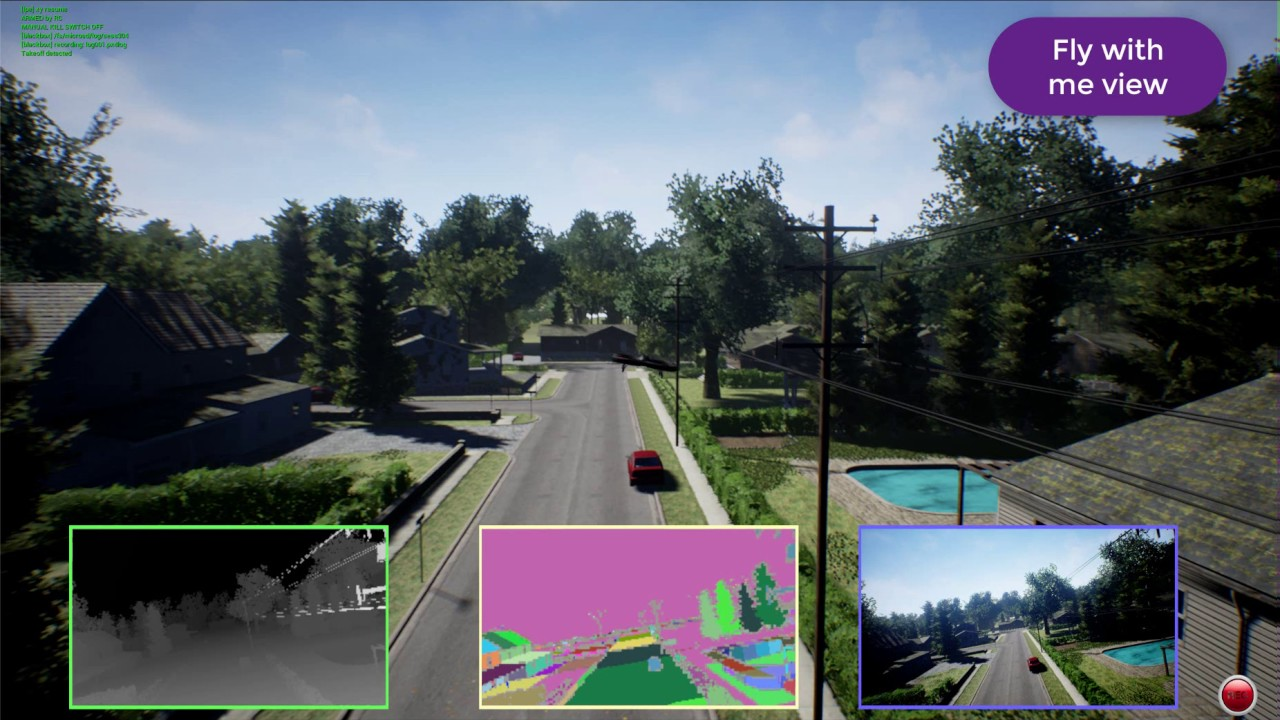
\includegraphics[width=0.4\textwidth]{airsim}
	\caption{Simulador Airsim}
	\label{fig-airsim}
\end{figure}

\subsection{Carla SIMULATOR}
Carla és un simulador gràfic elaborat en Unreal Engine aquest simulador té la finalitat de generar imatges en entorn fictici amb la màxima realitat possible per generar imatges que serveixin per a l'aprenentatge de xarxes neuronals capaces de conduir un cotxe autònom de forma segura tenint en compte els casos poc probables que no es podrien generar en un entorn físic. Aquest entorn compte amb les següents funcionalitats:

\begin{itemize}
  \item Simulació de cotxes
  \item Vista de mapa de profunditats
  \item Vista segmentada
  \item Simulació de tràfic
  \item Control dels actors amb scripts de python
\end{itemize}

\subsection{LESS}
LESS és un model de la redacció (com podem veure en la figura \ref{fig-lessradiacio}) efectuada en un objecte/terreny tridimensional per diferents raigs, generat a partir de tècniques de ray-tracing ens permet simular dades i imatges sobre escenes 3D realistes. Aquest model implementa un mètode de seguiment de fotons ponderats per simular el factor de reflectància bidireccional multi-espectral.

\begin{figure}[!h]
\centering
  	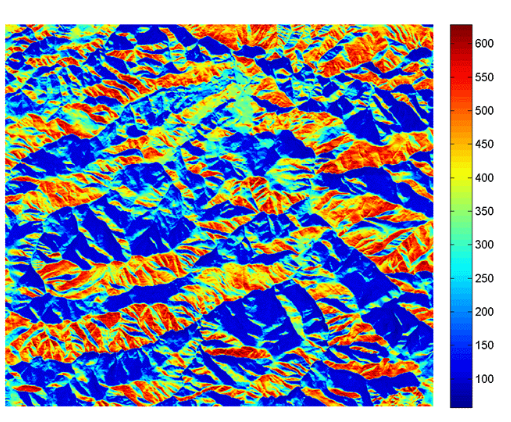
\includegraphics[width=0.4\textwidth]{lessradiacio}
	\caption{Exemple de resultats de radiació en un terreny}
	\label{fig-lessradiacio}
\end{figure}

\subsection{DIRSIG}

El model Digital Imaging i Remote Sensing Image Generation (DIRSIG) és un model de generació d'imatges sintètiques desenvolupat pel laboratori de Digital Imaging i Remote Sensing del Rochester Institute of Technology. El model pot produir imatges d'una sola banda, multiespectrals o hiperespectrals des del visible a través de la regió tèrmica d'infrarojos de l'espectre electromagnètic. Podem veure un exemple generat per DIRSIG en la figura \ref{fig-tacoma}.

\begin{figure}[!h]
\centering
  	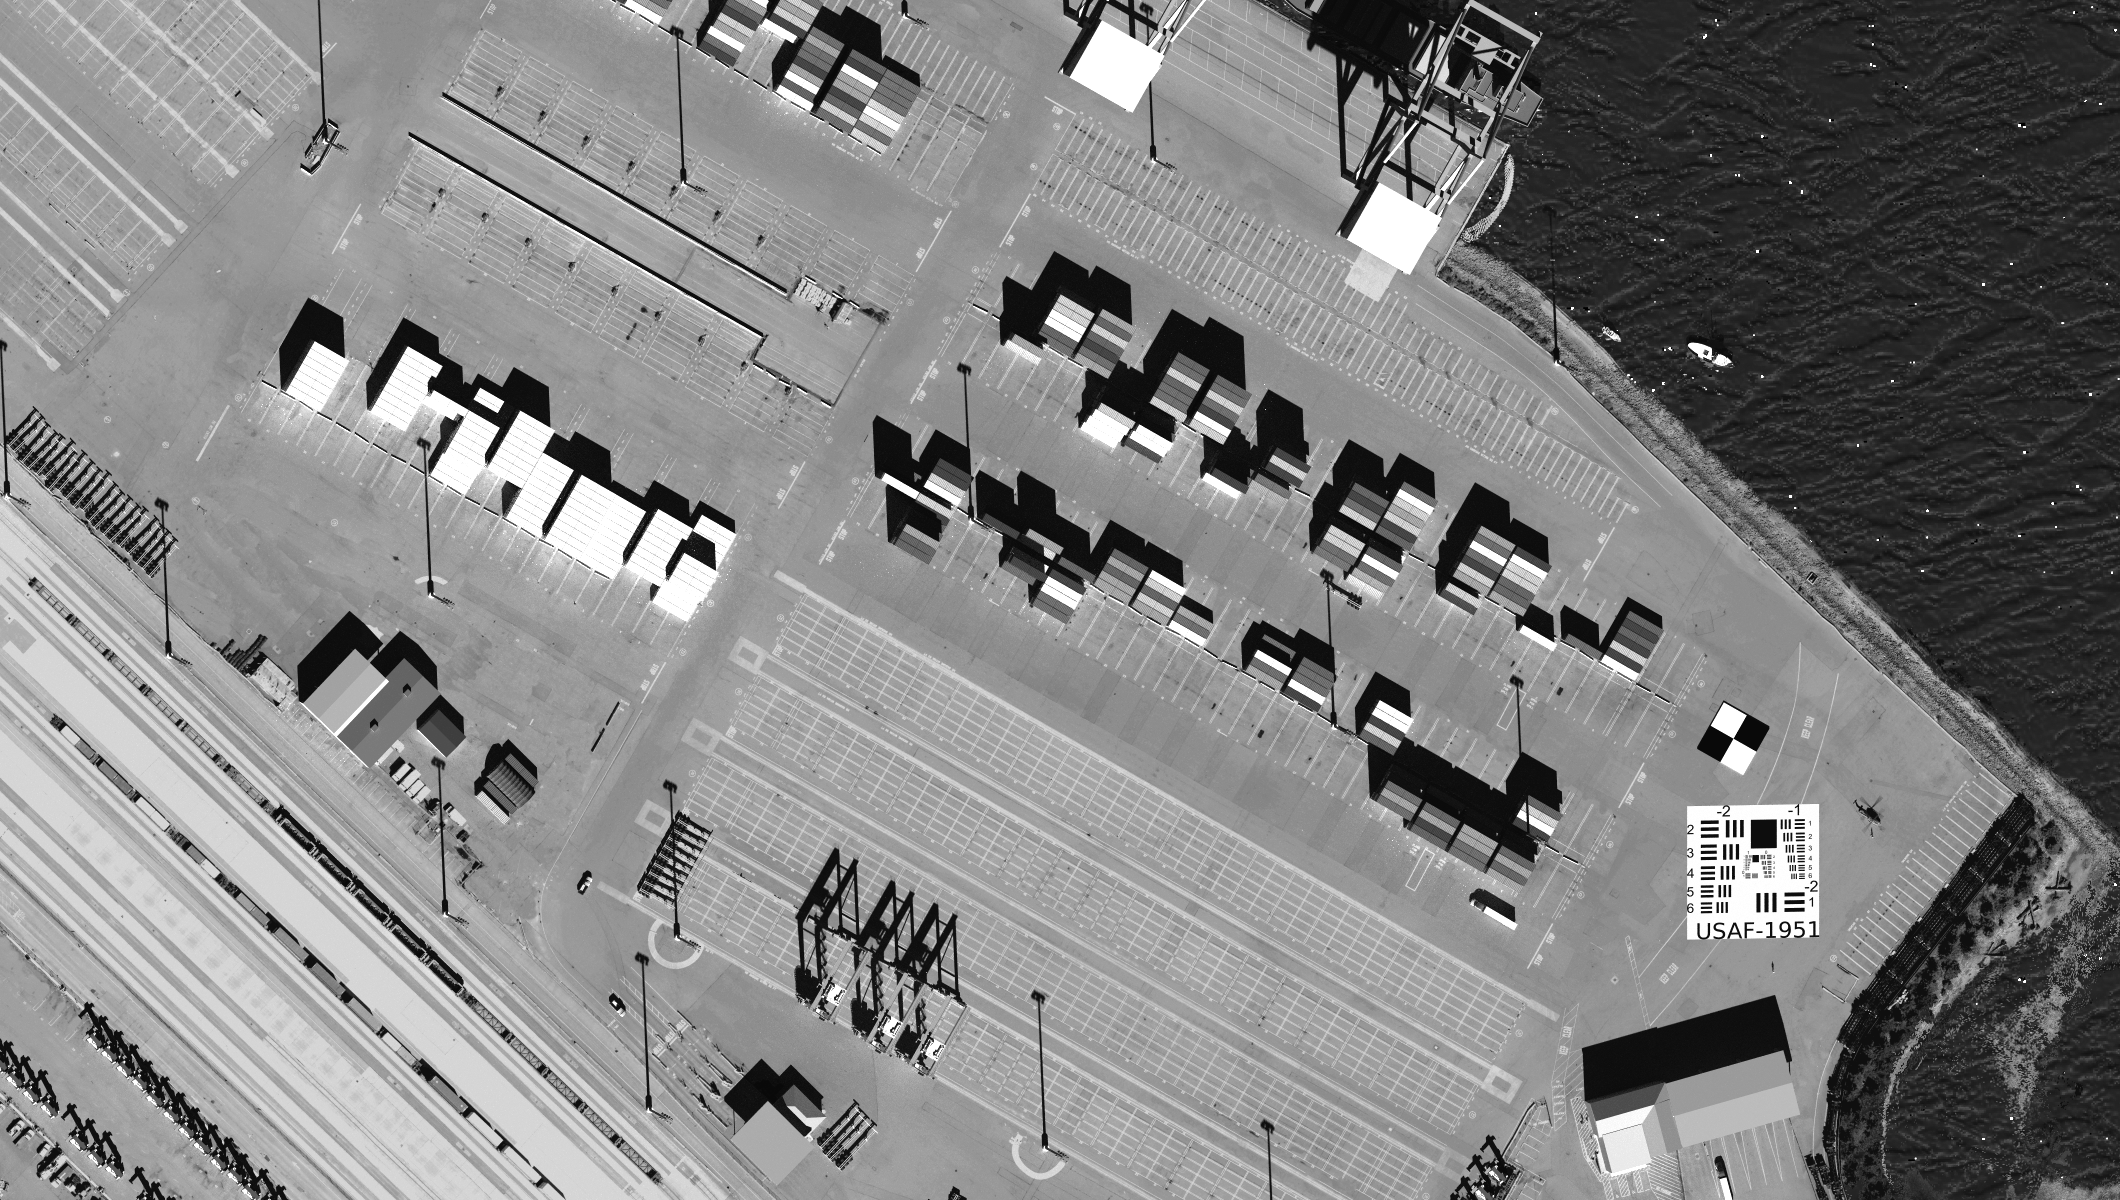
\includegraphics[width=0.4\textwidth]{tacoma}
	\caption{Frame del port de tacoma}
	\label{fig-tacoma}
\end{figure}

\subsection{Google Earth Engine}

Google Eath Engine és un projecte de Google dedicat a oferir les eines necessàries per tal de poder analitzar i visualitzar dades geospacials destinat a estudis acadèmics, institucions sense ànim de lucre, empreses i governs. Les característiques principals Google Earth Engine són:

\begin{itemize}
  \item Es pot treballar amb datasets de diferents satèl·lits com són LANDSAT, MODIS, SENTINEL, etc.
  \item Incorpora un entorn de treball per manipular la informació amb una extensa API que ens permet combinar imatges de diferents espectres, visualitzar-ho en el mapa del món, exportar-ho a Google Drive entre altres.
\end{itemize}

\section{Estructura del projecte}

Per tal de determinar l'estructura del nostre projecte s'han estudiat vàries alternatives vistes a l'apartat \ref{estatart} en les quals es pot veure com estan organitzats altres projectes similars. En aquest apartat veurem l'estructura de diferents projectes amb l'objectiu de decidir l'estructura del projecte i diferents llibreries.

\subsection{AirSim} 

AirSim està compost per múltiples mòduls escrits en diversos llenguatges com es pot veure a continuació:

\begin{itemize}
  \item \textbf{AirLib (C++)}: Mòdul per a Unreal Engine que proporciona les classes bàsiques per comunicar-se mitjançant el protocol RCP i control dels vehicles simulats.
  \item \textbf{DroneServer (C++)}: Servidor per rebre ordres de Dron mitjançant RCP.
  \item \textbf{DroneShell (C++)}: Client de consola per enviar ordres al mòdul de dron.
  \item \textbf{PythonClient (Python)}: Client que envia ordres mitjançant RCP, també incorpora codi per al tractament, segmentació d'imatges, etc.
  \item \textbf{SGM (C++)}: Codi per tractar imatges i generar les vistes segmentada i stereo.
  \item \textbf{Unity (C\# i C++)}: Demostració en el motor gràfic Unity, incorpora una sèrie de mòduls per Unity per visualitzar la informació d'AirSim.
  \item \textbf{Unreal Engine (C++)}: Demostració en el motor gràfic Unreal Engine, incorpora una sèrie de mòduls per Unreal Engine per visualitzar la informació d'AirSim.
\end{itemize}

\subsection{Carla SIMULATOR}

Carla SIMULATOR està compost per múltiples mòduls com podem veure en la figura \ref{fig-carlamodules} escrits en diversos llenguatges com es pot veure a continuació:

\begin{figure}[!h]
\centering
  	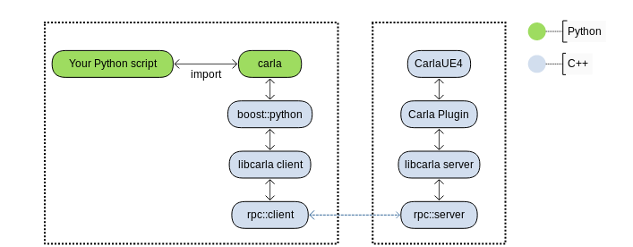
\includegraphics[width=0.5\textwidth]{carlamodules}
	\caption{Relació entre els mòduls de Carla}
	\label{fig-carlamodules}
\end{figure}

\begin{itemize}
 \item \textbf{LibCarla (C++)}: Llibreria principal de Carla
 \item \textbf{Unreal (C++)}: Motor gràfic amb el plugin de carla, que incorpora totes les funcionalitats afegides a Unreal.
 \item \textbf{PythonAPI (Python)}: API que ens permetrà enviar comandes al mòdul de Carla que fa de servidor, aquest api serveix per crear scripts propis.
\end{itemize}


\subsection{Estructura escollida}

Analitzant diversos projectes de característiques similars s'ha decidit per una estructura pròpia com podrem veure en la figura \ref{fig-dronsimulatormodules} podent reutilitzar alguns dels petits mòduls open-source d'altres projectes. S'ha pres aquesta decisió a causa del fet que els altres projectes es basen en la creació terrenys predefinits mitjançant l'entorn d'Unreal, contrari a la finalitat d'aquest projecte en el qual es volen elaborar de forma automàtica terrenys a partir de dades reals.

\begin{figure}[!h]
\centering
  	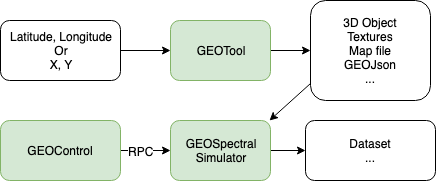
\includegraphics[width=0.45\textwidth]{structuretfg}
	\caption{Estructura DronSimulator}
	\label{fig-dronsimulatormodules}
\end{figure}

En el nostre projecte constarà d'aquests mòduls:

\begin{itemize}
  \item \textbf{GEOTool (Python)}: Aquest mòdul té la finalitat de donar les eines necessàries per a l'obtenció i adaptació de les dades proveïdes per webservices estàndard en l'àmbit de l'obtenció de dades geogràfiques amb l'objectiu de poder importar-les en qualsevol motor gràfic, podent generar diferents capes d'informació per als terrenys descarregats.
  \item \textbf{ScriptAPI (Python)}: API que ens permetrà fer scripts en Python per tal de controlar la càmera en l'entorn gràfic. D'aquesta forma també ens permetrà l'obtenció d'imatges en l'entorn Unreal Engine.
  \item \textbf{Unreal Engine Simulator (C++)}: Incorporarà tot el motor gràfic i connectors necessaris per a la comunicació amb els fitxers generats amb el mòdul GEOTool, visualització de dades, obtenció d'imatge, etc.
\end{itemize}

\section{Mòdul GeoTools}

Mòdul generat en Python amb l'objectiu d'obtenir informació de mapes d'elevacions, ortofotos, etc. Amb l'objectiu posterior de fer un tractament d'aquestes dades per la generació de terrenys tridimensional i informació en format visible per tal de poder visualitzar-ho en un motor gràfic de tipus Unreal, Unity, OpenGL, etc.

\subsection{Obtenció de dades}

Amb l'objectiu d'obtenir dades geogràfiques s'ha optat per la comunicació amb els estàndards proposats per l'Open Geospatial Consortium\cite{ogc}: Web Map Service\cite{wms} encarregat de posar a disponibilitat dades d'imatge com poden ser ortofotos d'una zona geogràfica seleccionada i Web Coverage Service\cite{wcs} encarregat de retornar informació referent a les elevacions de terreny en una zona geogràfica concreta. Per tal d'obtenir dades es fan peticions HTTP a les direccions web oferides per distintes institucions que segueixen els estàndard anomenats, en aquest cas s'ha realitzat proves amb l'Institut Cartogràfic i Geològic de Catalunya\cite{icgc}.

\subsubsection{Fitxer de configuració}

Per tal de determinar quines dades volem obtenir i de quins webservices l'aplicació accepta per paràmetre un fitxer de configuració en format JSON que ens permet determinar diferents propietats de les dades que demanarem com es pot veure en l'apèndix \ref{appendix:geotoolconfig}. En aquest fitxer es pot configurar els següents paràmetres:

\begin{itemize}
  \item \textbf{Type}: Fa referència al tipus de coordenades que li passarem, pot ser latlong o xy en el primer cas farà la corresponent transformació al format UTM (xy)
  \item \textbf{Coordinates}: Coordenades sobre les quals volem fer la petició en el format indicat en el camp type. Si s'escull "xy" es definirà els atributs x, y en cas d'escollir "latlong" definirem els atributs lat, long.

  \item \textbf{Dimensions}: En aquesta secció escollirem les dimensions que volem que es demanin en les peticions per tal de mantenir la mateixa zona geogràfica.
  \begin{itemize}
    \item Bbox: Aquestes seran les dimensions de la zona que volem obtenir amb les que es calcularà els límits que delimitaran la zona.
    \item Texture: Aquesta serà la resolució que obtindrem per les diferents textures.
  \end{itemize}

  \item \textbf{cellsize}: Mida de cada pixel en metres.
  \item \textbf{meshStep}: Número que indica la quantitat de punts que desitgem saltar a la malla (Per defecte 1). Més informació a la secció \ref{qualitat}.
  \item \textbf{Wcsurl}: URL al webservice que ens donarà les dades d'altures.
  \item \textbf{Outputwcs}: Nom de sortida del fitxer generat per les altures
  \item \textbf{Formatwcs}: Format del fitxer generat per les altures. Disponibles: raw, obj (Objecte 3D)

  \item \textbf{Wmsrequests}: Array amb cada una de les peticions que farem a diferents WMS per tal d'obtenir vàries imatges
  \begin{itemize}
    \item Url: URL al webservice WMS.
    \item Layers: capa o capes que volem obtenir d'aquests webservice.
    \item Output: Nom del fitxer de sortida.
    \item OutputFormat: Format del fitxer de sortida. Disponibles: JPG
  \end{itemize}
  
  \item \textbf{offset}: Objecte de dos components que ens indica el desplaçament en píxels aplicat a les coordenades.
\end{itemize}

\subsection{Estructura de GEOTool}
{
\LARGE TODO
}
\subsection{Generació de Terrenys a partir dun mapa d'altures}
En aquesta secció s'explicarà les diverses formes que s'han optat per generar terrenys que puguin ser interpretats en diferents motors gràfics.

\subsubsection{Format RAW}
El format RAW és un format pla que es basa en guarda en valors de 16 Bytes totes les altures en format binari tenim com a referència del mar el valor 128, i afegits en el fitxer un darrere de l'altre. Aquest format és acceptat per al creador de terrenys d'Unreal i Unity, però té certes limitacions de dimensions que s'han de complir especificades a l'editor en crear el terreny que fa que es perdi el control de la malla generada, les coordenades de textura no coincideixen amb la textura que es vol aplicar al terreny. Motius pels quals s'ha optat per afegir la generació de l'objecte 3D en format estàndard definit nosaltres l'objecte com es podrà veure en l'apartat \ref{mesh3d}, ja que aquestes limitacions fan que es facin vàries adaptacions no estàndards perquè es pugui visualitzar correctament.

\subsubsection{Generació de malla 3D}
\label{mesh3d}
Per tal d'importar terrenys en els motors gràfics s'ha optat per generar una malla 3D en format Wavefront obj\cite{wavefrontobj} format compatible amb qualsevol editor 3D, motor gràfic, etc. Aquest format dóna la llibertat per tal de controla la distància entre els vèrtexs, on s'aplicarà la textura i quines seran les normals dels vèrtexs fent que el terreny sigui suavitzat.
\\
\\
Com que el tractament amb bucles és lent s'ha realitzat tots els càlculs amb la llibreria NumPy aprofitant l'eficiència que incorpora aquesta llibreria amb el càlcul de matrius pel qual s'ha adaptat el problema com podem veure en el codi disponible en l'annex \ref{appendix:generateobj}.
\\
\\
Per la generació d'objectes cal definir 4 tipus d'objectes:

\begin{itemize}
  \item \textbf{Vèrtex}: Són cada un dels punts en el món, van definits pels índexs segons llegui'm la graella d'elevacions, es multipliquen per un K (Distancia entre els vèrtexs segons la distància que ens indiqui el mapa d'elevacions obtingut).

  \item {
    \textbf{Vèrtex de textura}: Vèrtex amb dos components x, y compresos entre el 0 i 1 que indican la correspondència entre els punts d'una textura i la malla en la qual es vol aplicar aquella textura. Aquestes propietats es calcularien amb les equacions \ref{equation:u} i \ref{equation:v}.
    \begin{equation}
    \label{equation:u}
    u = f(columna) = columna / (ample - 1)
    \end{equation}
    \begin{equation}
    \label{equation:v}
    v = f(fila) = 1 - (fila / (altura - 1))
    \end{equation}
  }

  \item \textbf{Normal del vèrtex}: Vectors que ens indica la direcció en la qual es reflecteix la llum per a cada vèrtex de l'objecte. Per tal de calcular aquestes normals cal el pas previ de calcular les normals de cada cara, aquestes no seran introduïdes al fitxer final, ja que aquestes les genera'n els motors per defecte segons l'ordre en el qual indiquem els vèrtexs de les cares com es veurà més endavant.
  \begin{itemize}
    \item {
       Generació de normals de cares: Per tal de generar les normals d'una cara un cop sapiguem la relació entre les cares se seguirà el patró vist en la figura \ref{fig-normalcara} on seguirem l'equació \ref{equation:u} per al càlcul de la normal de la cara. $\dot{\vec{A}}$ i, realitzarem el producte vectorial $\vec{C} = \vec{B}*\vec{A}$ i per últim normalitzarem el vector $\vec{Normal} = \frac{\vec{C}}{\mid\vec{C}\mid}$.
    }
    \item {
      Generació de normals en els vèrtexs: Per tal de generar el vector normal per a cada vèrtex utilitzarem l'estructura que es pot veure en la figura \ref{fig-normalvertex} aplicant la següent formula a cada vèrtex on V correspon als vèrtexs i F a les cares de la figura \ref{fig-normalvertex}:
      \begin{equation}
      \vec{NormalV} = \vec{F1} + \vec{F2} + \vec{F3} + \vec{F4} + \vec{F5} + \vec{F6}
      \end{equation}
      \begin{equation}
      \vec{NormalV} = \frac{\vec{NormalV}}{\mid\vec{NormalV}\mid}
      \end{equation}
    }
  \end{itemize}

  \item \textbf{Cares}: En aquest punt determinarem quina és la unió dels vèrtexs per tal de generar les diferents cares de la malla, en aquesta implementació s'ha decidit per fer triangulació, és a dir, per cada quadrat de la nostra malla generarem 2 cares triangulars. És important generar les cares mantenint l'ordre dels vèrtexs contrari a les agulles del rellotge, d'aquesta forma els motors gràfics determina'n que la normal de la cara apuntarà cap dalt visualitzant correctament la malla 3D.
\end{itemize}

\begin{figure}[!h]
\centering
  	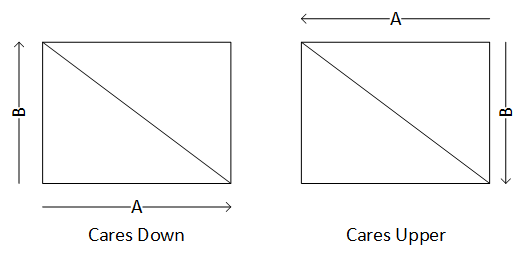
\includegraphics[width=0.4\textwidth]{caranormal}
	\caption{Patró per càlcul de normals en les cares}
	\label{fig-normalcara}
\end{figure}

\begin{figure}[!h]
\centering
  	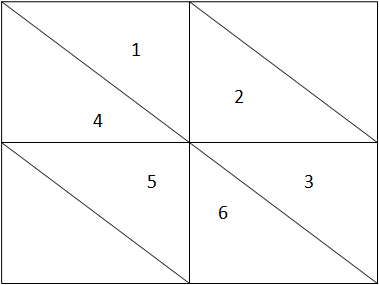
\includegraphics[width=0.2\textwidth]{vertexnormal}
	\caption{Patró per càlcul de normals en un vèrtex}
	\label{fig-normalvertex}
\end{figure}

Un cop realitzat el procés de generació l'aplicació haurà generat una malla que podem obrir en qualsevol editor com podem veure en la figura \ref{fig-meshlab}

\begin{figure}[!h]
\centering
  	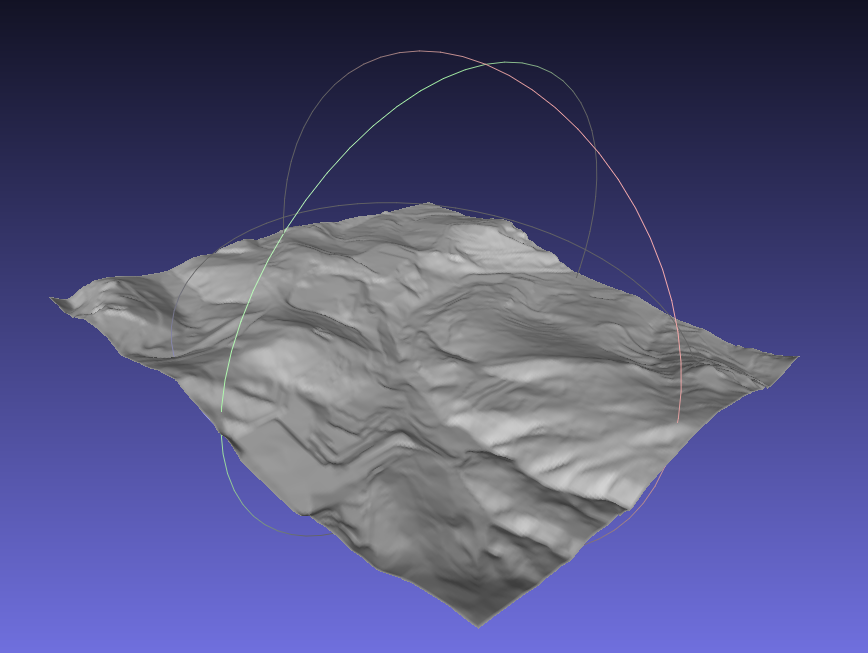
\includegraphics[width=0.35\textwidth]{mesh_example_meshlab}
	\caption{Malla d'un terreny visualitzada en l'aplicació MeshLab}
	\label{fig-meshlab}
\end{figure}

\subsubsection{GEOJson associat al terreny}
Per tal de poder localitzar el terreny que hem generat en altres aplicatius que treballin amb dades geoespacials o en el mateix simulador d'Unreal s'hi ha incorporat la generació d'un GEOJson que ens indica la zona al qual pertany el fitxer generat. Podem veure un exemple de GEOJson a l'annexa \ref{appendix:geojson}.

\subsection{Temps de generació}
En aquest apartat s'analitzaran les dues versions implementades i es podrà veure les diferencies en temps de generació. Aquest és un punt important per futures implementacions en les quals es desitjaria implementar un visor en temps real del món carregant nova informació segons l'usuari es mogui pel món. 
\\
En la figura \ref{fig-meshtime} veiem els temps per la versió amb bucles for i la versió implementada amb NumPy, com es pot veure quant realitzem la implementació utilitzant la llibreria NumPy s'aconsegueix reduir el temps en 24x per la mida 500*500 gran això és degut al fet que NumPy està optimitzada per a paral·lelitzar el tractament de dades de forma vectorial.

\begin{figure}[!h]
\centering
  	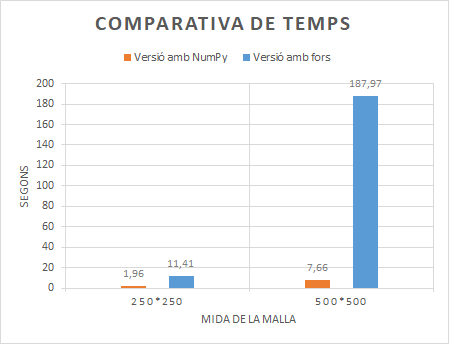
\includegraphics[width=0.4\textwidth]{meshtime}
	\caption{Gràfic amb el temps de generació d'una malla segons la mida}
	\label{fig-meshtime}
\end{figure}

\subsection{Qualitat}
\label{qualitat}
En aquest apartat es mirarà la forma en la qual reduïm la qualitat del terreny i veurem els resultats obtinguts tant qualitativament (diferència visual) com quantitativament (mida en bytes).

Per tal de fer aquesta reducció fem salts de la mida que volem reduir (2,4,8,16,...) en la nostra matriu de punts. Les proves s'han fet amb un terreny de 300x300 pixels. 

Com podem veure en la figura \ref{fig-qualitatmegas} al reduir la quantitat de punts reduïm de forma exponencial la mida que ocupa en disc dur fent més lleugera la càrrega dels fitxers per l'entorn d'Unreal.
\\
\\
Com podem veure en la figura \ref{fig-qualityvisual} es pot visualitzar la pèrdua de qualitat agafant com a referència la muntanya del fons en la que veiem com es perd la definició en el pic. Podem considerar visualment que quant configurem ''meshStep'' en 1 i 2 la pèrdua qualitativa no és apreciable, a partir de 4 es comença a apreciar lleugerament, finalment en els nivells 8 i 16 es pot veure la major pèrdua en la que es pot apreciar els pics en forma de punxa en compte de la serralada que es veu amb el step més baix.

\begin{figure}[!h]
\centering
  	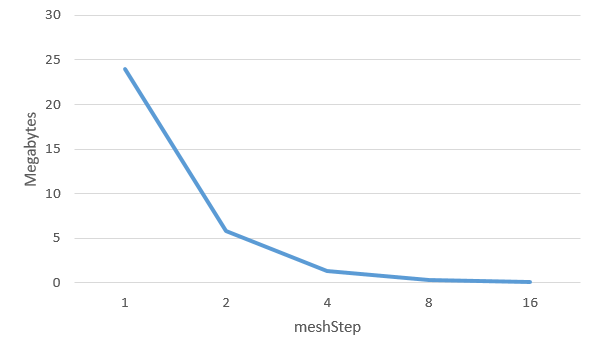
\includegraphics[width=0.4\textwidth]{qualitatmegas}
	\caption{Gràfic de mida en disc dur dels fitxers .obj per un terreny de 300x300}
	\label{fig-qualitatmegas}
\end{figure}

\begin{figure}[!h]
\centering
  	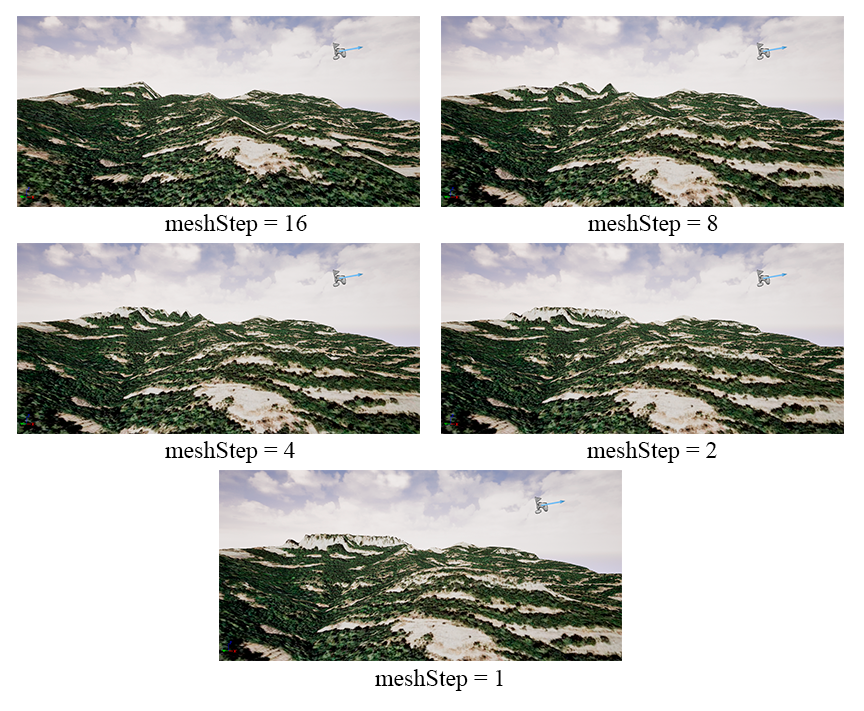
\includegraphics[width=0.5\textwidth]{quality/quality}
	\caption{Comparativa visual dels efectes produits pel nivell de qualitat}
	\label{fig-qualityvisual}
\end{figure}


\section{Mòdul: Simulador}

En aquesta secció explicarem els diferents punts dels quals es compon el mòdul de simulació amb el que se cerca l'objectiu de posar a disposició una eina que ens permeti simular un viatge amb un vehicle genèric per sobre d'un terreny obtenint imatges des de diferents càmeres configurades anteriorment.

\subsection{Visualització i control del Vehicle}
Aquesta part serà l'encarregada de donar la interfície per moure un vehicle genèric pel nostre món simulat, aquest vehicle es configurarà amb una sèrie de càmeres que es podran visualitzar en la pantalla i generar imatges de cada una d'elles afegint la possibilitat de obtenir múltiples vistes d'una mateixa localització. Podem veure una vista zenital en la figura \ref{fig-montserratir}.

\begin{figure}[!h]
\centering
  	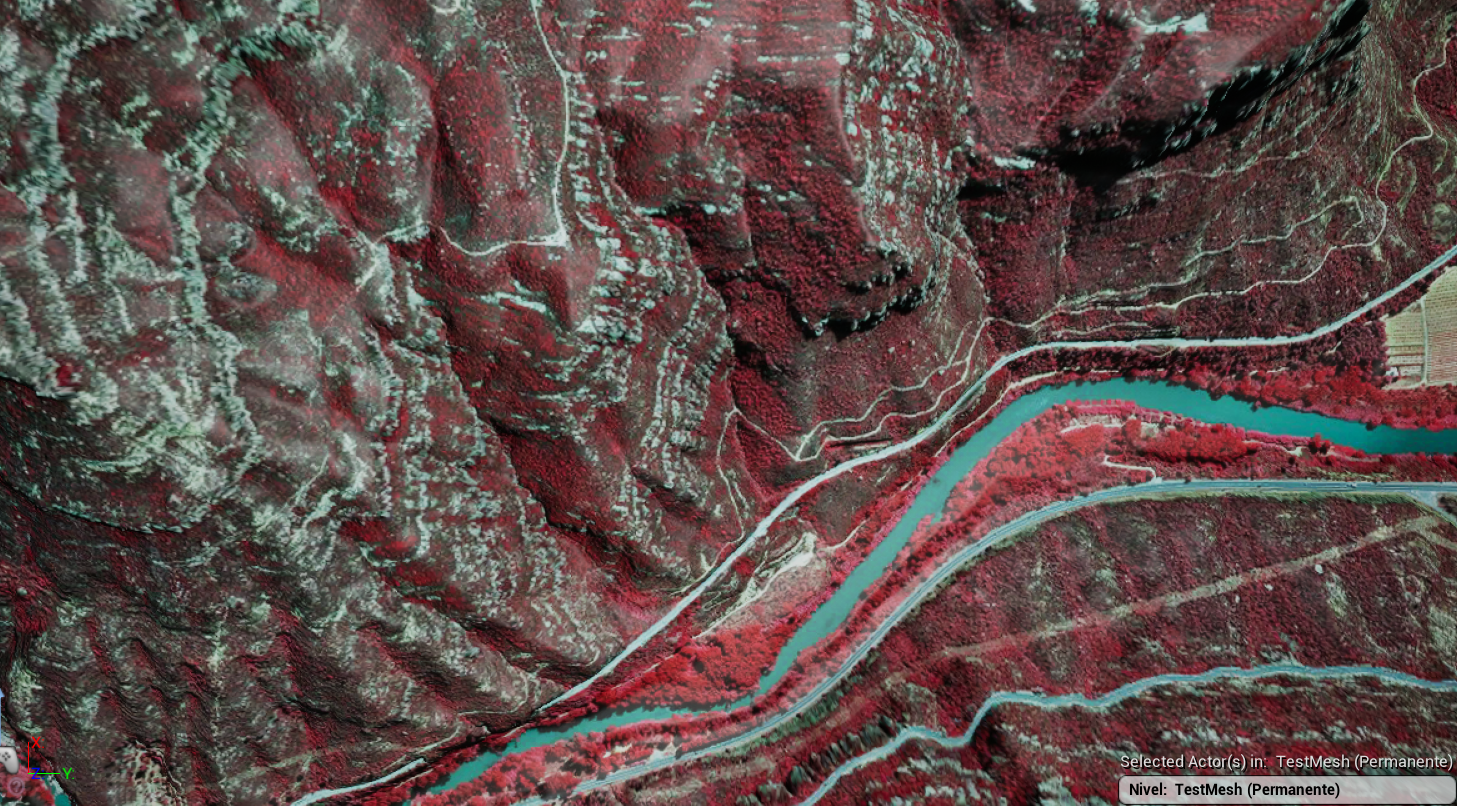
\includegraphics[width=0.5\textwidth]{cenitalviewir}
	\caption{Vista zenital infraroja de Montserrat}
	\label{fig-montserratir}
\end{figure}

\subsubsection{Control remot}
Per tal de controlar remotament el vehicle s'implementa una comunicació utilitzant el protocol RPC (Remote Procedure Call) en concret s'utilitza la llibreria Rpclib\cite{rpclib} per a C++. Aquest servidor s'implementarà en el mòdul d'Unreal, la gestió del servidor RPC es fa mitjançant una classe (AVehiclePawn) que podem heretar de forma que permetrà donar la interfície necessària per a controlar un Vehicle en concret es podran realitzar les següents accions:

\begin{itemize}
\item Inicialitzar/parar el servidor RPC: Inicialitzem el servidor prement la tela Y al simulador d'Unreal i l'aturem amb la tecla U.
\item Canviar la posició del vehicle
\item Canviar la rotació
\item Demanar que es generin imatges d'una de les càmeres
\end{itemize}

L'assignació de les funcionalitats es fa en la funció ''void BindFunctions(rpc::server* server)'' la qual rep la instància del servidor, aquesta funció es pot sobreescriure per afegir posteriorment en classes heretades més funcionalitat com es pot veure en l'annexa \ref{appendix:extendrpc}. Per defecte la classe AVehiclePawn ens permet cridar a les següents funcions RPC:

\begin{itemize}
\item setLocation(double x, double y, double z): Enviem la localització en la qual volem que és situí el nostre vehicle.

\item setLookAt(double x, double y, double z): Enviem el vector amb la posició en el món que volem visualitzar, d'aquesta forma calcularem en quin punt del simulador es ha de mantenir la vista de la càmera.

\item setLocationAndLookAt(double x, double y, double z, double lx, double ly, double lz): Funció que crida d'un a les dues anteriors.

\item setCameraLookAt(int cameraId, double x, double y, double z): Funció que canvia la direcció en la que mira la càmera que l'indiquem.

\item getImage(int idCamera, std::string path): Ens permet indicar de quina càmera i on volem guardar la imatge.
\end{itemize}

\subsubsection{Visualització del cel}
Per tal d'implementar el cel hem utilitzat un modul natiu d'Unreal que ens permet generar una sphere en la que es renderitza un cel aquest cel té diversos paràmetres ajustables que ens permet determinar la posició del sol en aquell moment, el nivell de brillantor de les estrelles, la quantitat de núvols, etc. 
\\\\
Això dona la possibilitat de generar imatges sintètiques en diferents moments del dia amb diferents il·luminacions, el que permetrà generar datasets més complexos. D'altra banda això comportarà que haurem d'aplicar textures sense ombres per tal que aquestes siguin generades per al motor d'Unreal. Podem veure un exemple de diferents hores del dia a la figura \ref{fig-sky}.

\begin{figure}[!h]
\centering
  	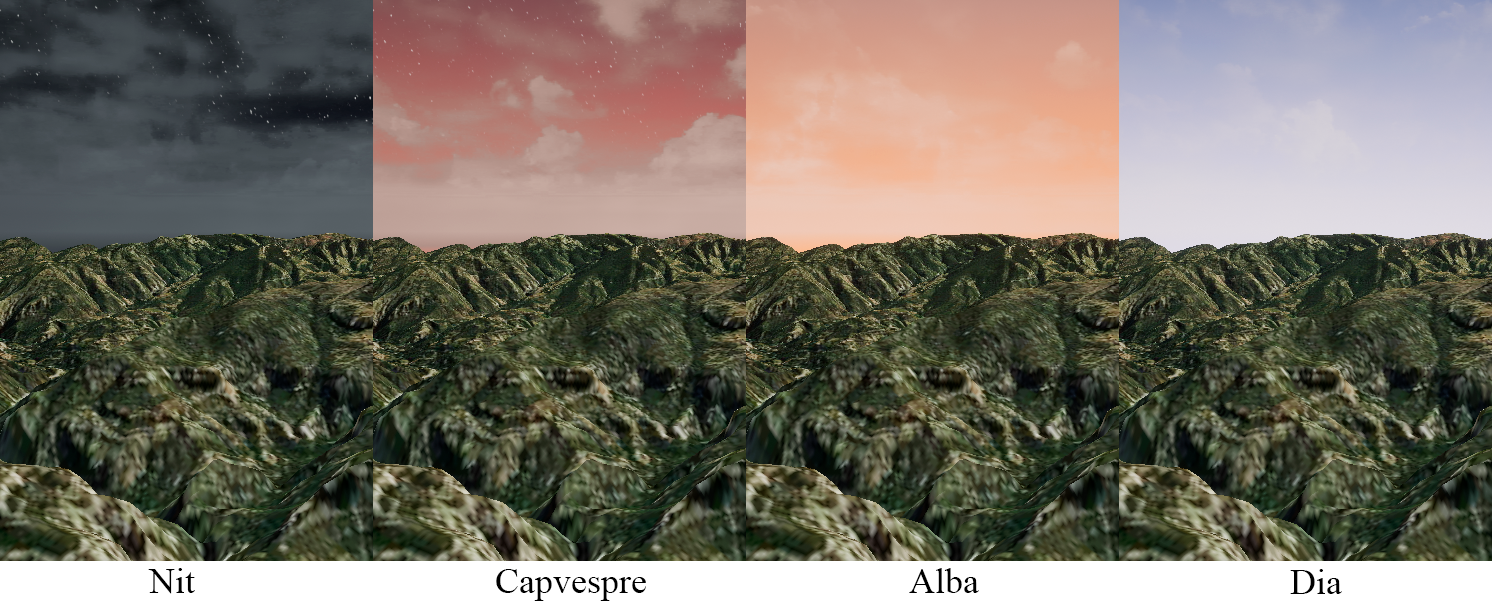
\includegraphics[width=0.48\textwidth]{sky/sky}
	\caption{Exemple de cels}
	\label{fig-sky}
\end{figure}

\subsection{Terreny}
El terreny és carregat mitjançant codi obtenint el fitxer .obj i processant aquest fitxer per tal de generar una malla en temps d'execució generant un UProceduralMesh\cite{uprocedural} d'Unreal, per tal de realitzar aquesta tasca es té en compte que Unreal treballa amb un sistema de coordenades invertit respecte al model UTM en el qual l'eix Y es troba invertit a conseqüència d'això es ha de realitzar la reflexió en l'eix Y els objectes fent la correspondència que pertoqui en cada moment entre el món real i el món simulat.
\\
\\
Aquesta malla és carregada al món i representada per la classe ''MapChunk'' al qual se li assignarà el material dinàmic que contindrà les textures carregades de les diferents visualitzacions que desitgem podent visualitzar qualsevol de les imatges que preparem en format imatge per al terreny com poden ser textures RGB, Infraroig, multi espectral, etc.

\subsection{Visualització del terreny}
En aquest apartat veurem els resultats obtinguts a partir de terrenys 3D generats pel mòdul GEOTool i l'aplicarem diverses visualitzacions de fonts com són textures o shaders obtinguts per diversos medis, en concret les vistes RGB i infraroig són obtingudes de l'Institut Cartogràfic de Catalunya, les dades multiespectrals les obtenim de l'explorador EO Browser\cite{eobrowser} i la informació de profunditat l'obtenim d'aplicar un shader a l'escena.
\\
\\
Com podem veure en la figura \ref{fig-bands} hem aplicat a un terreny corresponent a ''Sales de Pallars'' diferents bandes multiespectrals obtingudes pel satèl·lit Sentinel 2\cite{sentinel2}. Les tres primeres bandes B02, B03 i B04 corresponen a bandes de colors, la banda B05 correspon al canvi ràpid de reflectància que fa la vegetació en un rang proper a l'infraroig, la banda B08 obté informació NIR\cite{nir} i per últim veiem la banda B09 capaç de detectar vapors d'aigua.

D'aquesta forma amb aquestes bandes podem obtenir informació composta per diversos espectres que podem aplicar a diversos àmbits. En la figura \ref{fig-spectralindexes} es poden veure alguns exemples, entre ells podem veure índexs com són:

\begin{itemize}
\item 
{
	NVDI\cite{ndvi}: Basat en la combinació de les bandes (B08 - B04)/(B08 + B04), índex utilitzat per veure l'estat del conreu.
}
\item
{
	Moisture index\cite{moisture}: Basat en la combinació de les bandes (B8A - B11)/(B8A + B11), indica la proporció de precipitació que es necessita per tal de satisfer les necessitats de la vegetació.
}
\item
{
	NDWI\cite{ndwi}: Basat en la combinació de les bandes (B03 - B08)/(B03 + B08), índex que s'utilitza per determinar l'estrès hídric de la vegetació, saturació de la humitat en el terra o realitzar delimitacions de masses d'aigua com a llacs o embassaments.
}
\end{itemize} 

En l'última vista de la figura \ref{fig-spectralindexes} es pot veure la de profunditat o proximitat utilitzada per algoritmes de reconstrucció 3D amb monocular stereo, prevenció de col·lisions, algoritmes de multiview stereo, etc.

\begin{figure*}[!h]
\centering
  	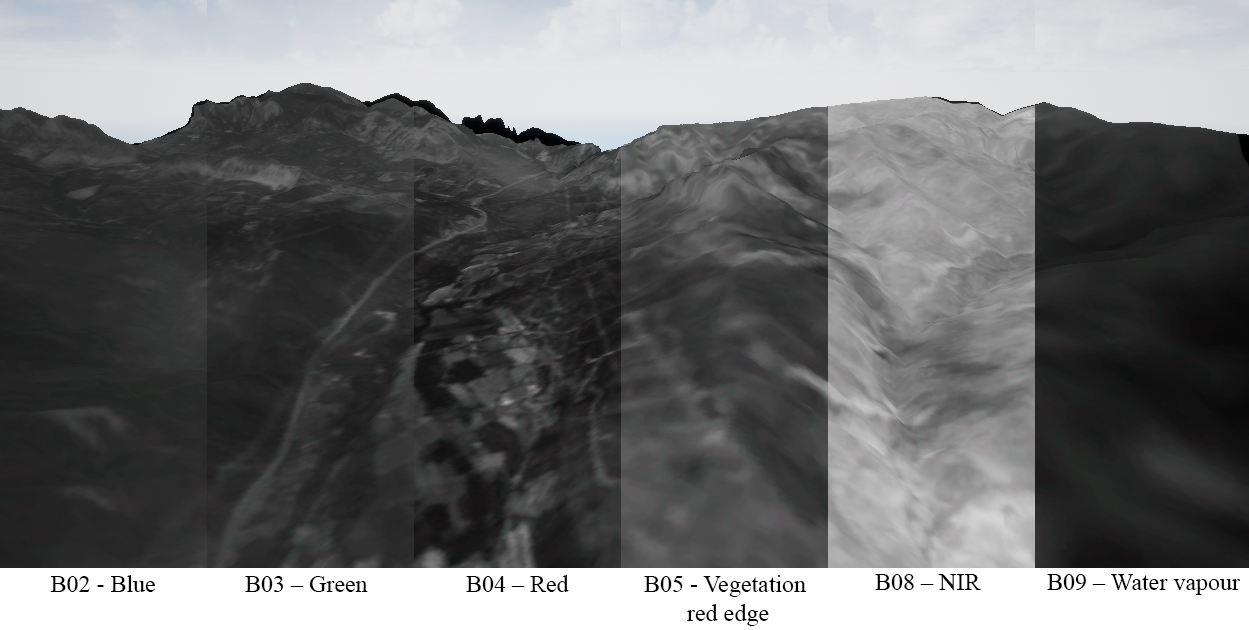
\includegraphics[width=1\textwidth]{multispectral/bands}
	\caption{Vista de Sales de Pallars en 6 bandes diferents}
	\label{fig-bands}
\end{figure*}

\begin{figure*}[!h]
\centering
  	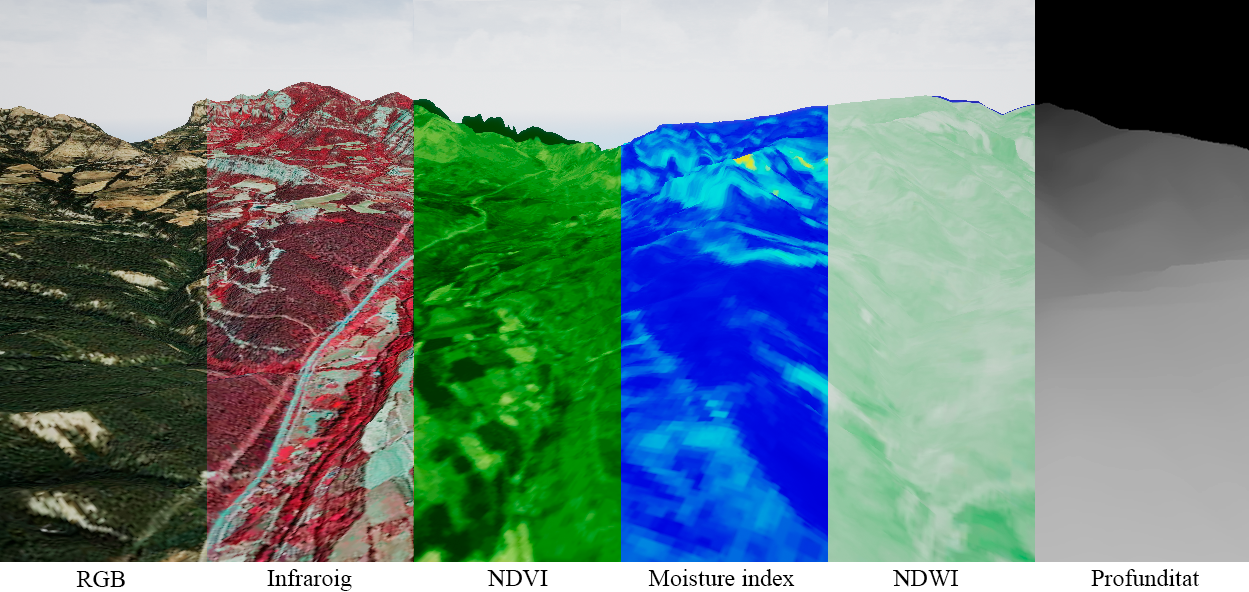
\includegraphics[width=1\textwidth]{multispectral/spectralindexes}
	\caption{Vista de Sales de Pallars en RGB, Infraroig, NDVI, Moisture, NDWI i profunditat}
	\label{fig-spectralindexes}
\end{figure*}

\subsection{Interacció amb el simulador}
Per tal d'interaccionar amb el simulador s'han definit les següents tecles:

\begin{itemize}
\item A,W,S,D: Per moure'ns en el simulador.
\item Q,E: Per rotar la vista.
\item Y: Inicia el servidor RPC.
\item U: Para el servidor RPC.
\item H: Mostra/oculta la visualització del vehicle.
\item K: Guarda en un fitxer la vista actual de la segona càmera.
\end{itemize}

\section{Mòdul d'Scripting}
En aquest apartat explicarem i veurem els principals punts del mòdul d'scripting en el qual podrem gestionar el simulador de forma que podrem recrear viatges llegint fitxers de trajectòries, generar imatges, generar soroll a les trajectòries, etc.

\subsection{Trajectòries}
El mòdul d'scripting permet fer vols llegint trajectòries creades en el món real (adaptant-les al nostre format) o generades sintèticament d'aquesta forma podem recrear en el simulador la trajectòria feta anteriorment podent reproduir tants cops com vulguem aquesta, això ens permetrà fer diverses proves amb diferents visualitzacions del terreny. Per aquesta finalitat s'ha generat el fitxer que expliquem a la secció \ref{file-trajectories}.

\subsubsection{Fitxer de trajectòries}
\label{file-trajectories}
En aquest apartat explicarem com està formatjat el fitxer de trajectòries i el fitxer per posicionar la càmera. Els fitxers estaran en format CSV i seran llegits des de mòdul GEOControl per a indicar al simulador les posicions del vehicle i cap a quina posició del món mira tant el vehicle com les càmeres.

El fitxer que controla al vehicle està compost pels següents camps:

\begin{itemize}
\item Time: Temps en mil·lisegons d'ençà que comença el script.
\item x: Posició X en format UTM.
\item y: Posició Y en format UTM.
\item z: Posició Z en format UTM.
\item LookX: Posició X a la que mirem en format UTM.
\item LookY: Posició Y a la que mirem en format UTM.
\item LookZ: Posició Z a la que mirem en format UTM.
\end{itemize}

Per tal de controlar a on miran les cameras tindrem un altre fitxer composat per els camps:

\begin{itemize}
\item Time: Time en milisegons des de que comença el script.
\item cameraId: Id de la camera que volem modificar.
\item LookX: Posició X a la que mirem en format UTM.
\item LookY: Posició Y a la que mirem en format UTM.
\item LookZ: Posició Z a la que mirem en format UTM.
\item GetImage: Booleà de 0 o 1 en el que indiquem si volem generar una imatge d'aquesta càmera en aquell instant de temps.
\end{itemize}

Podem veure un exemple dels fitxers CSV a l'apèndix \ref{appendix:fitxerscsv} generats amb Excel.

\subsection{Simulació de soroll}
Ja que els vehicles tenen moviments inesperats a conseqüència de l'aire, l'asfalt entre d'altres s'ha implementat un generador de soroll aplicat a la trajectòria que volem reproduir d'aquesta forma podem generar imatges amb soroll i moviments inesperats. Aquest soroll s'ha implementat mitjançant un soroll gaussià en el qual utilitzem com a centre el punt al qual ens volem moure i una sigma petita (entre 0 i 1) que ens generarà un moviment lleuger.

\subsection{Generació de Datasets}
Un dels objectius d'aquest treball és la possibilitat de generar datasets d'imatges sintètiques amb dades generades per satèl·lits, per tal de poder generar datasets s'utilitza el camp GetImage vist a la secció \ref{file-trajectories} que ens generarà una imatge cada cop que trobi aquest camp.

En la figura \ref{fig-dataset} podem veure una petita mostra amb poques imatges d'un recorregut en el qual hem fixat que la càmera mires a un punt en concret que deixàvem enrere amb el transcurs del temps. 

\begin{figure}[!h]
\centering
  	\includegraphics[width=0.45\textwidth]{dataset/dataset}
	\caption{Conjunt d'imatges generades per GEOControl}
	\label{fig-dataset}
\end{figure}

\section{Conclusions}
En aquest projecte hem vist com hem pogut obtenir textures i mapes d'elevacions de fonts procedents de satèl·lits i convertir-les en informació 3D que pugui ser afegida a un motor gràfic com és Unreal Engine. S'ha tingut en compte aspectes com la velocitat en generar el model 3D on s'ha pogut veure com afecta llibreries com NumPy en el tractament de matrius accelerant aquest procés gràcies a la paral·lelització, s'ha pogut veure l'efecte que té quantitativament i qualitativament en les malles en reduir la quantitat de punts amb els quals es genera el model 3D necessari per a la renderització de models de grans dimensions.

Per la part del mòdul simulador hem pogut veure com podem visualitzar informació en un entorn 3D generat amb Unreal Engine. Es poden afegir càmeres a un vehicle simulat i veure des de diferents perspectives una mateixa informació per això s'ha creat un altre modulo que envia comandes al servidor RPC que s'ha implementat en Unreal Engine el qual pot moure, dir cap a on mira el vehicle, dir cap a on mira les càmeres i obtenir imatges d'aquestes càmeres.
S'han fet proves amb diverses visualitzacions provinents d'informació de satèl·lits com és el Sentinel 2 en el que s'ha pogut veure com és representa'n en el món simulat i quines utilitats té aquesta informació.

Per la part del mòdul d'scripting s'ha vist com es poden generar trajectòries reproduïbles en l'entorn simulat per tal de fer diversos viatges amb diferents informacions i extraure dades en forma de dataset. Aquestes trajectòries poden controlar diversos paràmetres del vehicle i càmeres indicant en quins punts es vol obtenir una imatge i de quina càmera. Per tal de simular el moviment a causa del vent o altres factors s'ha afegit un petit filtre com és la generació de soroll per tal de fer que se sacsegi el vehicle.


\section*{Agraïments}

\begin{thebibliography}{11}
\bibitem{agile}
Agile software development
\\ \url{https://en.wikipedia.org/wiki/Agile_software_development}
[19/02/2019]

\bibitem{kanban}
Kanban
\\ \url{https://www.iebschool.com/blog/metodologia-kanban-agile-scrum/} [19/02/2019]

\bibitem{trello}
Trello - \url{https://trello.com/} [19/02/2019]

\bibitem{airsim}
AirSim - \url{https://github.com/Microsoft/AirSim} [19/02/2019]

\bibitem{carla}
Carla SIMULATOR - \url{http://carla.org} [19/02/2019]

\bibitem{less}
LESS - \url{http://lessrt.org/} [11/04/2019]

\bibitem{dirsig}
Digital Imaging and Remote Sensing Image Generation - \url{http://dirsig.org/} [11/04/2019]

\bibitem{googleearth}
Google Earth Engine - \url{https://earthengine.google.com/} [20/05/2019]

\bibitem{unreal}
Unreal Engine - \url{https://www.unrealengine.com/en-US/what-is-unreal-engine-4} [09/03/2019]

\bibitem{ogc}
Open Geospatial Consortium (OGC) -  \url{http://www.opengeospatial.org/} [08/04/2019]

\bibitem{wms}
Web Map Service (WMS) -  \url{https://www.opengeospatial.org/standards/wms} [08/04/2019]

\bibitem{wcs}
Web Coverage Service (WCS) -  \url{https://www.opengeospatial.org/standards/wcs} [08/04/2019]

\bibitem{icgc}
Institut Cartogràfic i Geològic de Catalunya (ICGC) - \url{http://www.icgc.cat/ca/} [08/04/2019]

\bibitem{wavefrontobj}
Wavefront .obj file - \url{https://en.wikipedia.org/wiki/Wavefront_.obj_file} [09/04/2019]

\bibitem{rpclib}
RPC Lib - Modern mgspack-rpc for C++ - \url{http://rpclib.net/} [10/04/2019]

\bibitem{uprocedural}
Procedural Mesh Component - \url{https://wiki.unrealengine.com/Procedural_Mesh_Component_in_C%2B%2B:Getting_Started} [21/05/2019]

\bibitem{eobrowser}
EO Browser - \url{https://apps.sentinel-hub.com/eo-browser/} [25/05/2019]

\bibitem{sentinel2}
Sentinel 2 - \url{https://www.esa.int/esl/ESA_in_your_country/Spain/SENTINEL_2} [25/05/2019]

\bibitem{nir}
Tecnología NIR, sus Usos y Aplicaciones - \url{https://www.engormix.com/balanceados/articulos/tecnologia-nir-sus-usos-t32534.htm} [25/05/2019]

\bibitem{ndvi}
El NDVI o Índice de vegetación de diferencia normalizada - \url{https://geoinnova.org/blog-territorio/ndvi-indice-vegetacion/} [25/05/2019]

\bibitem{moisture}
Moisture index - \url{http://glossary.ametsoc.org/wiki/Moisture_index} [25/05/2019]

\bibitem{ndwi}
Cálculo del índice NDWI - \url{http://www.gisandbeers.com/calculo-del-indice-ndwi-diferencial-de-agua-normalizado/} [25/05/2019]

\end{thebibliography}

\appendix
\section*{Apèndix}

\setcounter{section}{1}

\subsection{JSON d'exemple per la configuració de GEOTool}
\label{appendix:geotoolconfig}
\lstinputlisting{geotoolconfig.json}

\subsection{Codi per la generació d'una malla 3D a partir d'un fitxer d'altures}
\label{appendix:generateobj}
\lstinputlisting[language=Python]{generateobj.py}

\subsection{GEOJson d'exemple}
\label{appendix:geojson}
\lstinputlisting{geojson.json}

\subsection{Codi d'exemple per estendre la funcionalitat RPC}
\label{appendix:extendrpc}

\lstset{language=C} 
\begin{lstlisting}
.h:
	virtual void BindFunctions(rpc::server* server) override;
	
.cpp:
void MyClass::BindFunctions(rpc::server* server)
{
	Super::BindFunctions(server);

	server->bind("nameOfFunction", [context_params](Variables...) {
		//MyCode
	});
}

\end{lstlisting}

\subsection{Fitxers CSV d'exemple per controlar el vehicle i les càmeres}
\label{appendix:fitxerscsv}

\begin{figure}[!h]
\centering
  	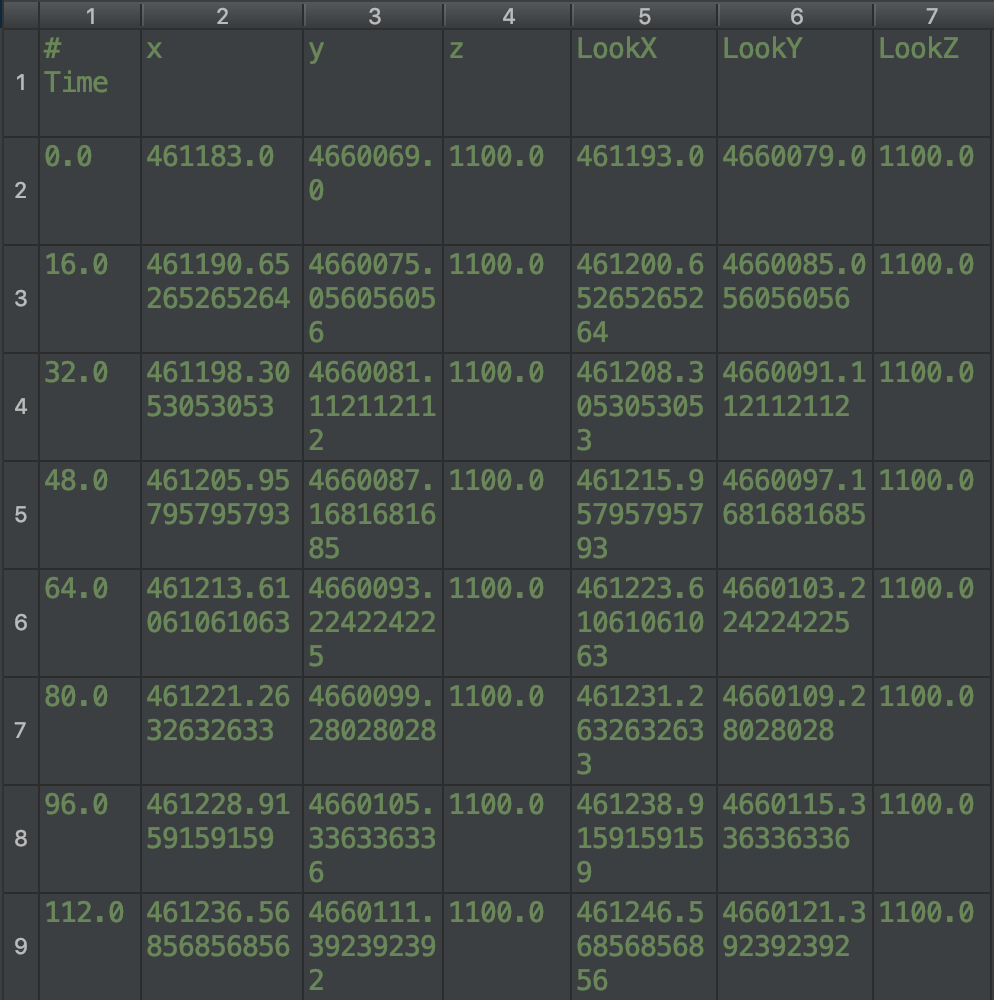
\includegraphics[width=0.45\textwidth]{fitxervehicle}
	\captionsetup{labelformat=empty}
	\caption{Fitxer CSV per controlar el vehicle}
	\label{fig-fitxervehicle}
\end{figure}


\begin{figure}[!h]
\centering
  	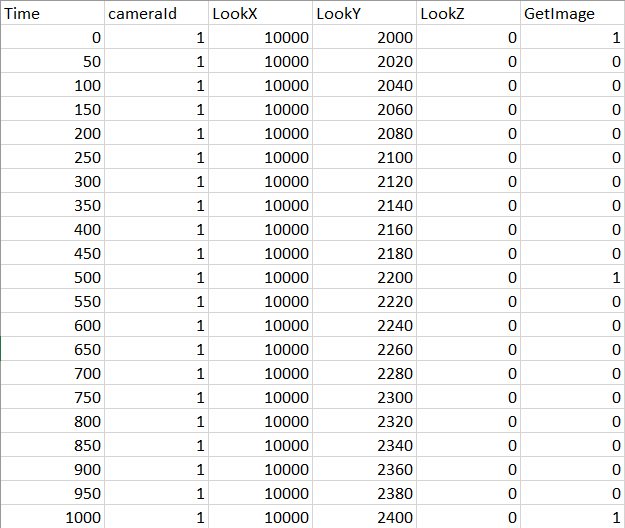
\includegraphics[width=0.45\textwidth]{fitxercameres}
  	\captionsetup{labelformat=empty}
	\caption{Fitxer CSV per controlar les càmeres}
	\label{fig-fitxercameres}
\end{figure}


\end{document}

